% Bloques de figuras para el reporte (Nivel 1).
% Requiere \usepackage{graphicx}. Colocar la carpeta figuras/ junto al .tex.
% Los pies son sugeridos: ajustar la redacción al estilo del reporte.

\begin{figure}[htbp]
  \centering
  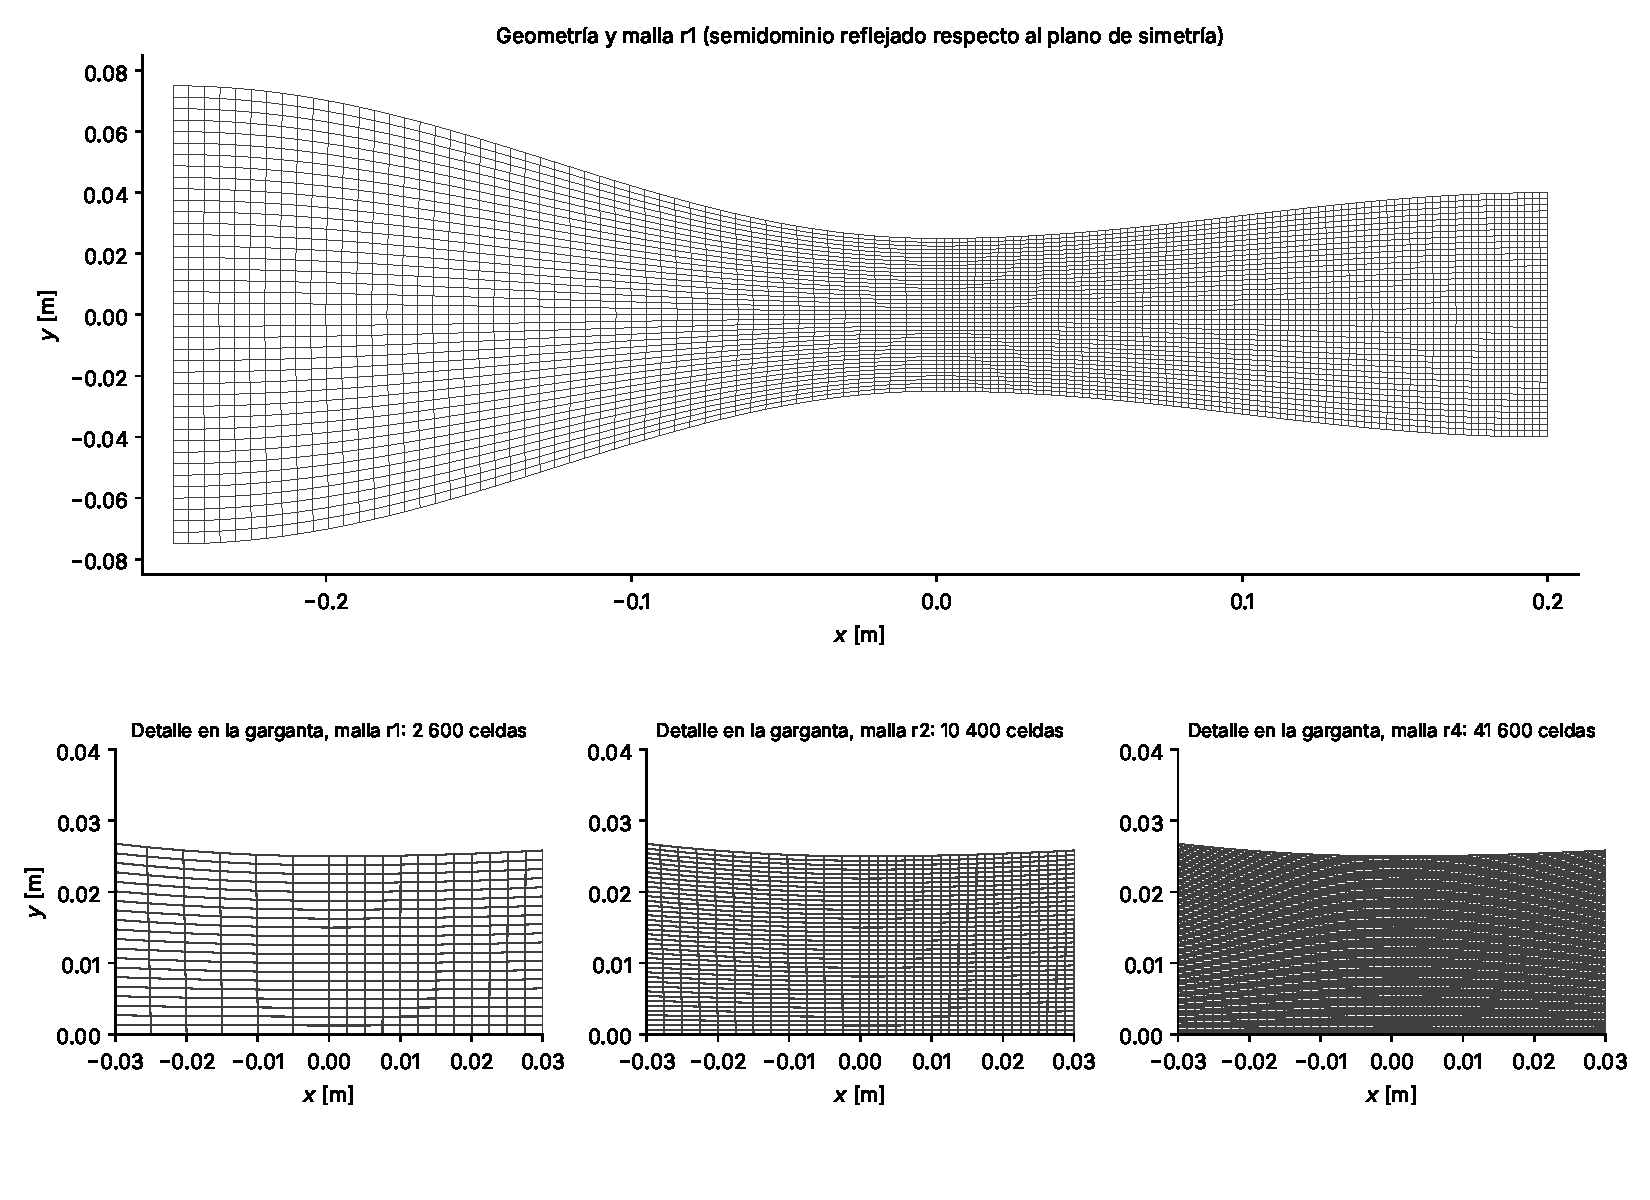
\includegraphics[width=\textwidth]{figuras/geometria_mallas.pdf}
  \caption{Geometría de la tobera y mallas estructuradas utilizadas. Arriba, malla r1 del semidominio reflejado respecto al plano de simetría. Abajo, detalle en la garganta para las mallas r1 (2\,600 celdas), r2 (10\,400) y r4 (41\,600).}
  \label{fig:geometria-mallas}
\end{figure}

\begin{figure}[htbp]
  \centering
  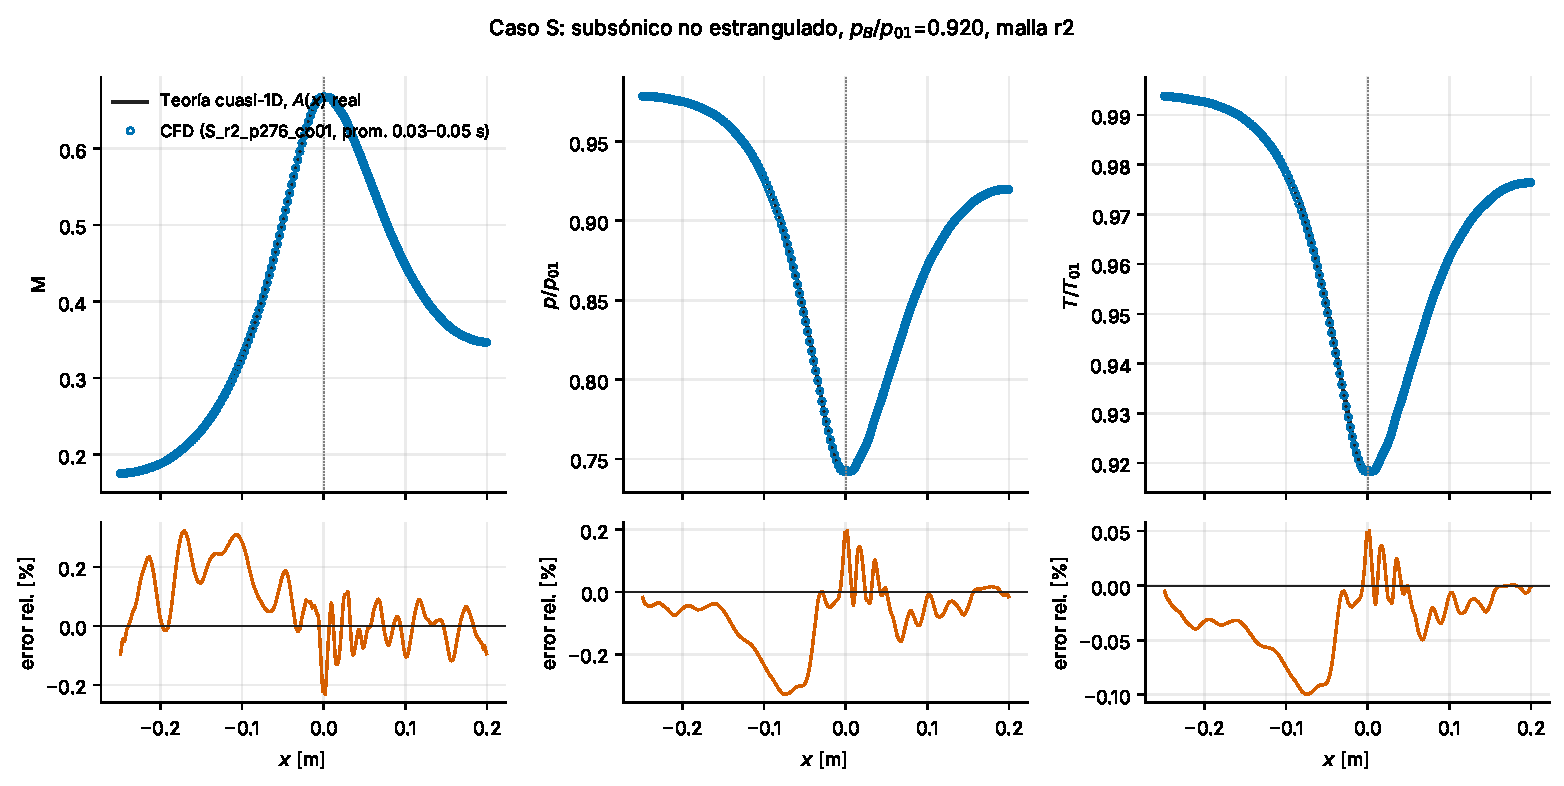
\includegraphics[width=0.85\textwidth]{figuras/perfiles_S_r2.pdf}
  \caption{Caso S (subsónico no estrangulado, $p_B=276$ kPa), malla r2. Perfiles de Mach, presión y temperatura a lo largo del eje, promediados en ventana de tiempo, contra la solución cuasi-unidimensional con la distribución real $A(x)$.}
  \label{fig:perfiles-S}
\end{figure}

\begin{figure}[htbp]
  \centering
  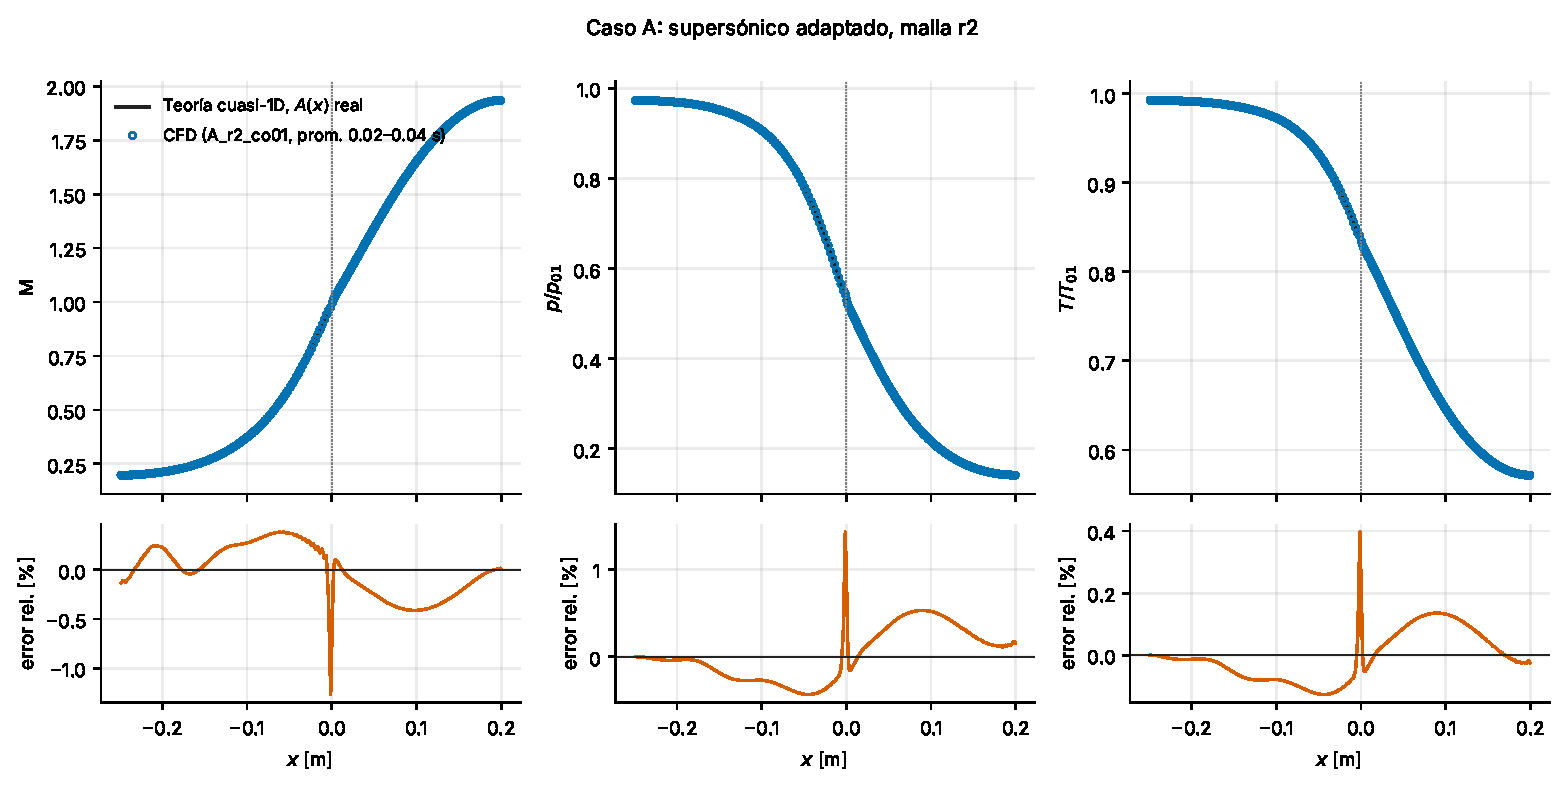
\includegraphics[width=0.85\textwidth]{figuras/perfiles_A_r2.pdf}
  \caption{Caso A (supersónico adaptado), malla r2. Perfiles CFD frente a la teoría cuasi-unidimensional (rama supersónica).}
  \label{fig:perfiles-A}
\end{figure}

\begin{figure}[htbp]
  \centering
  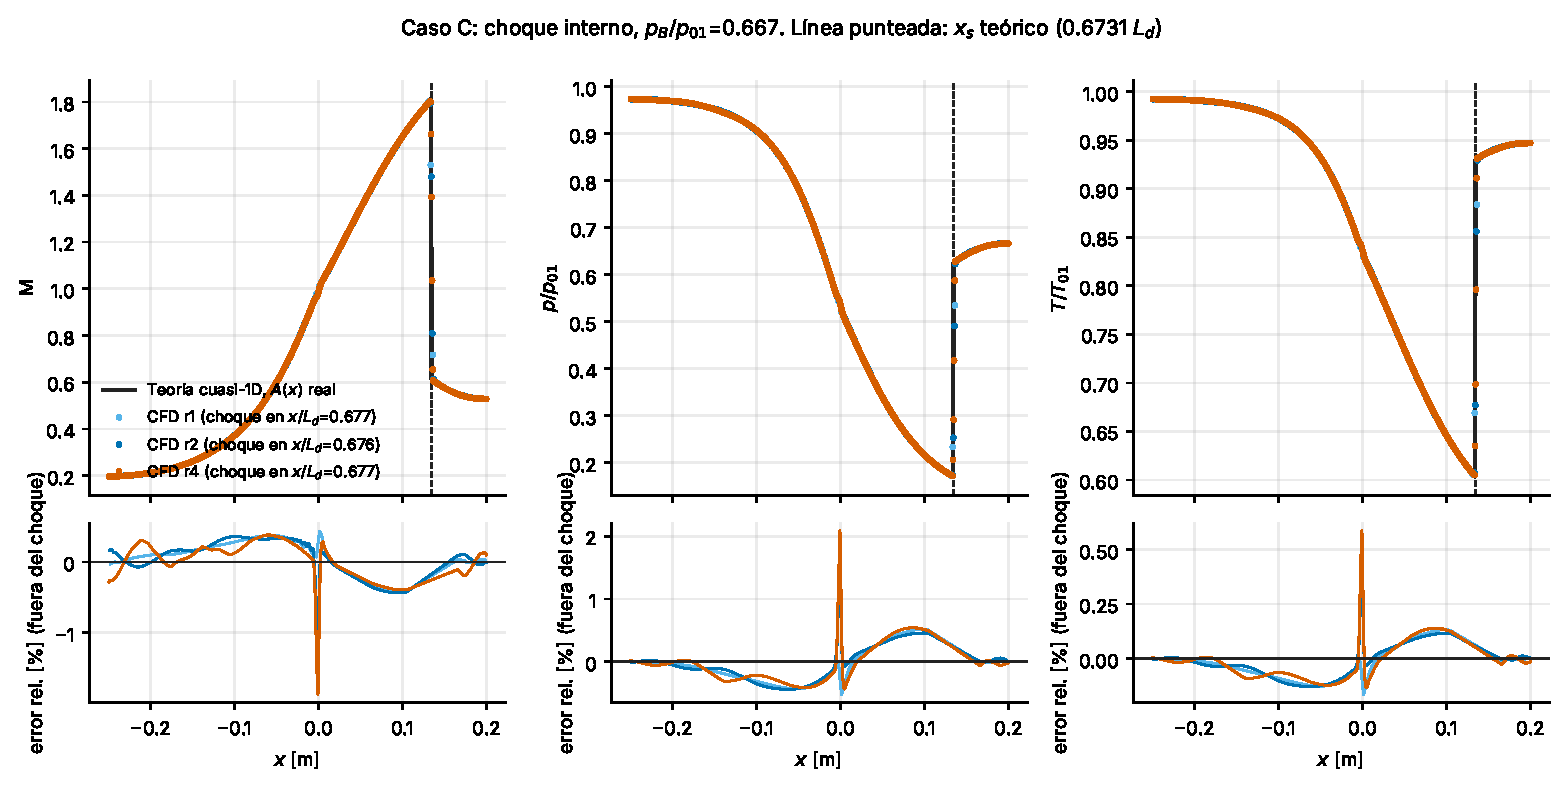
\includegraphics[width=0.85\textwidth]{figuras/perfiles_C_mallas.pdf}
  \caption{Caso C (choque interno, $p_B=200$ kPa). Perfiles obtenidos con las mallas r1, r2 y r4 frente a la teoría; el choque se ubica en $x_s/L_d\approx0.676$ en las tres mallas (teoría: 0.673).}
  \label{fig:perfiles-C}
\end{figure}

\begin{figure}[htbp]
  \centering
  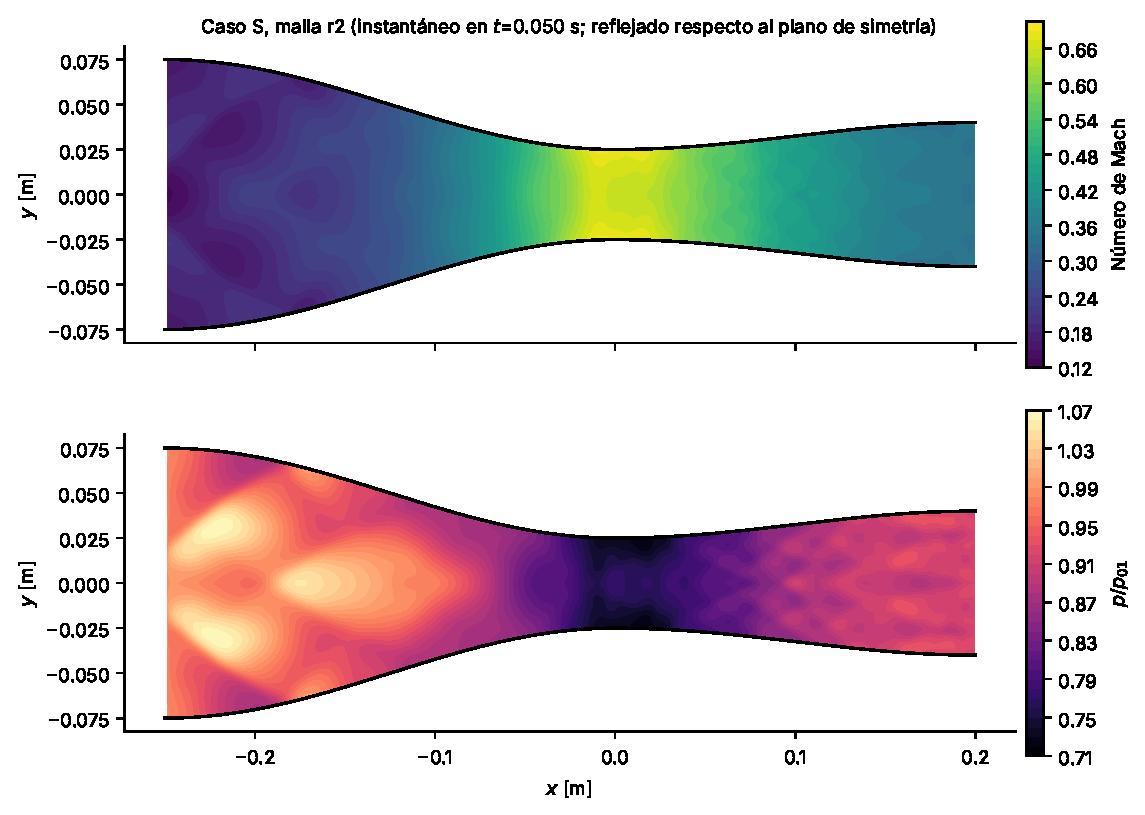
\includegraphics[width=0.8\textwidth]{figuras/mapas_S_r2.pdf}
  \caption{Caso S, malla r2: campos de número de Mach y de presión adimensional $p/p_{01}$ (semidominio reflejado).}
  \label{fig:mapas-S}
\end{figure}

\begin{figure}[htbp]
  \centering
  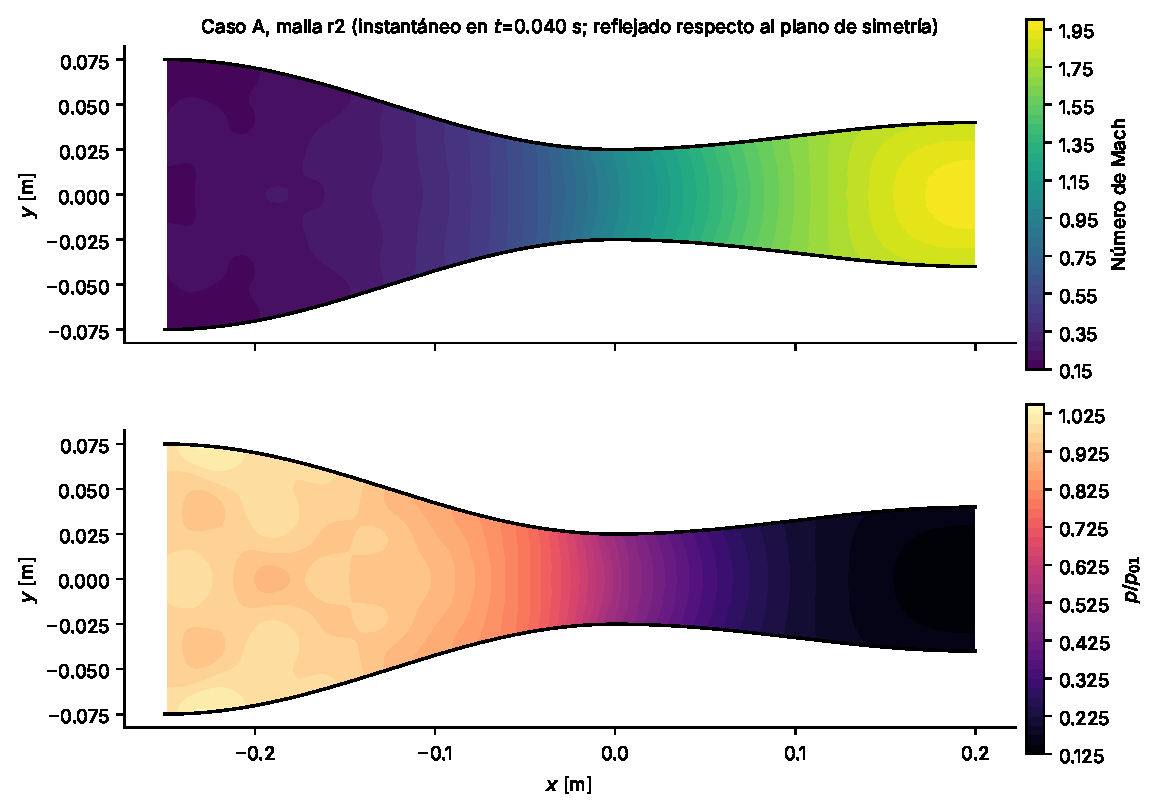
\includegraphics[width=0.8\textwidth]{figuras/mapas_A_r2.pdf}
  \caption{Caso A, malla r2: campos de número de Mach y de presión adimensional $p/p_{01}$.}
  \label{fig:mapas-A}
\end{figure}

\begin{figure}[htbp]
  \centering
  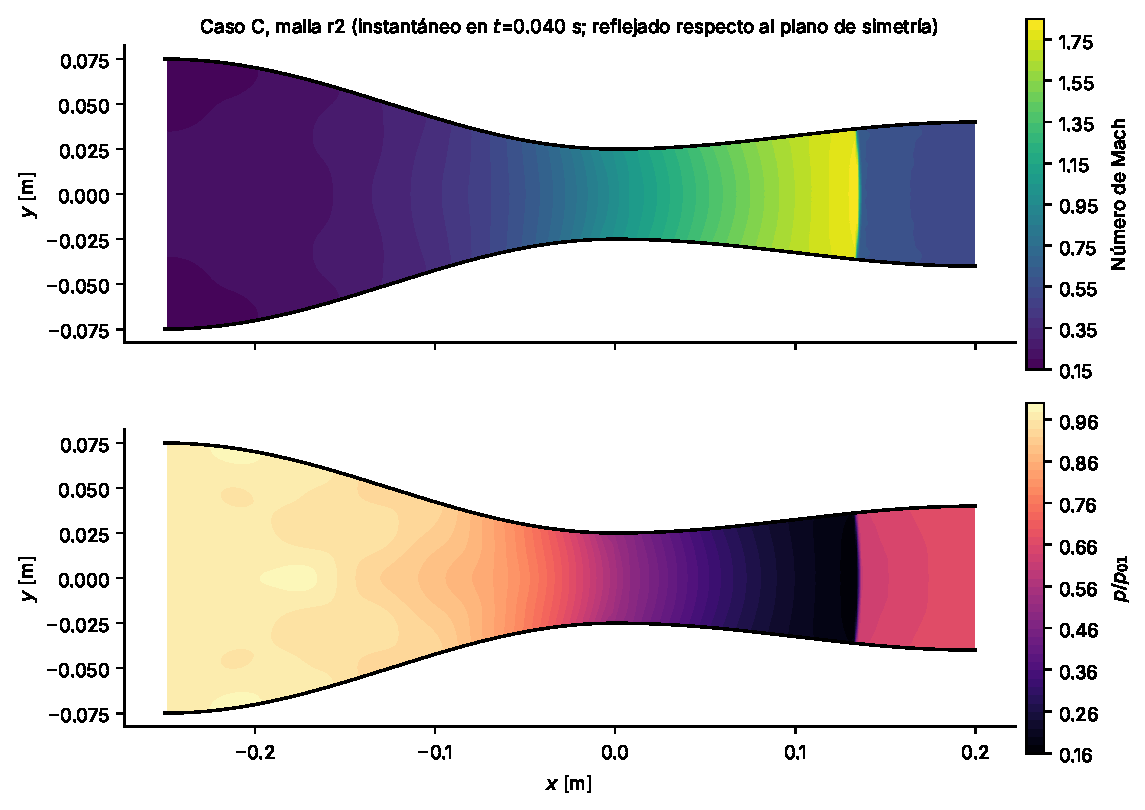
\includegraphics[width=0.8\textwidth]{figuras/mapas_C_r2.pdf}
  \caption{Caso C, malla r2: campos de número de Mach y de presión adimensional $p/p_{01}$. Se aprecia el choque normal en el divergente y el flujo subsónico aguas abajo.}
  \label{fig:mapas-C}
\end{figure}

\begin{figure}[htbp]
  \centering
  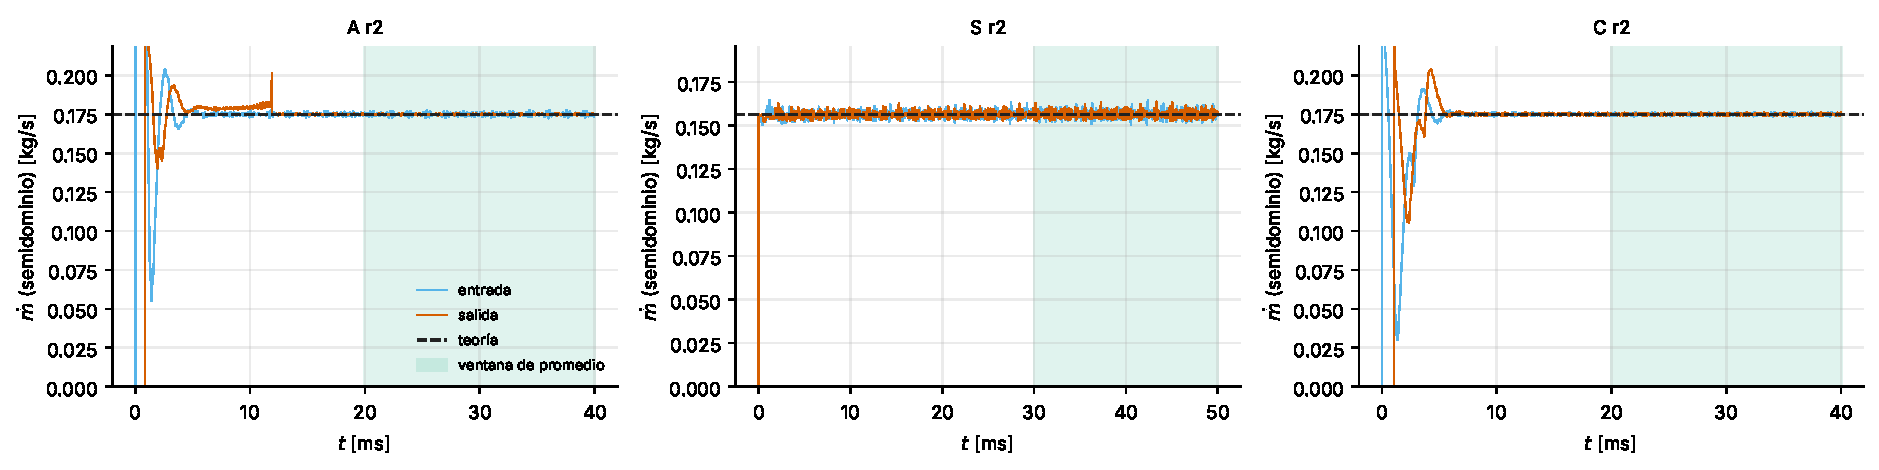
\includegraphics[width=\textwidth]{figuras/gasto_historias.pdf}
  \caption{Historias del gasto másico de entrada y de salida para los casos de referencia. El balance de masa cierra dentro de los criterios de convergencia una vez superado el transitorio inicial.}
  \label{fig:gasto-historias}
\end{figure}

\begin{figure}[htbp]
  \centering
  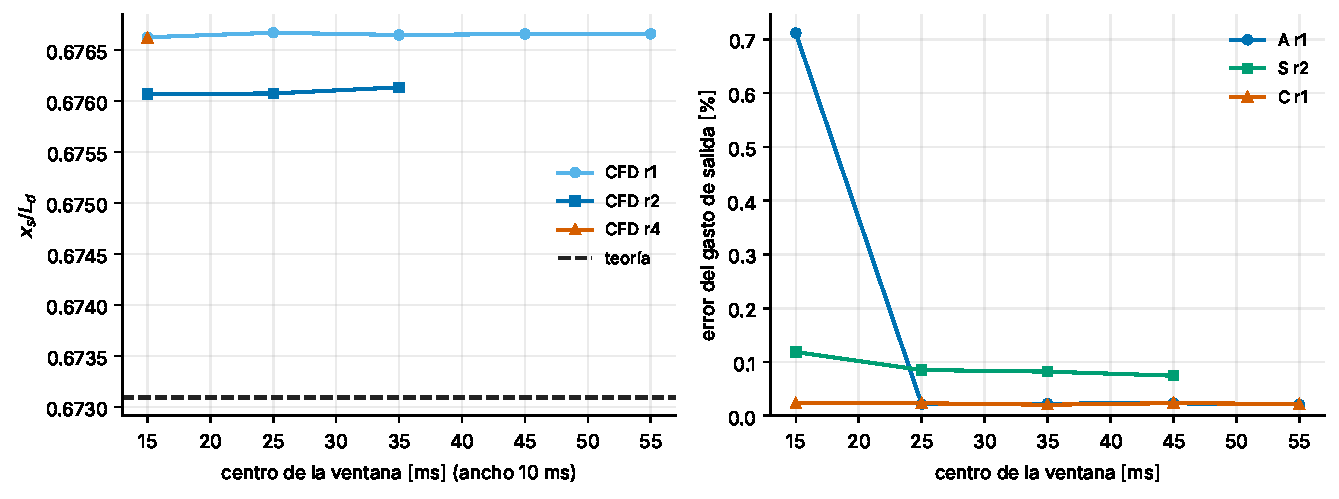
\includegraphics[width=\textwidth]{figuras/convergencia_ventanas.pdf}
  \caption{Convergencia por ventanas de tiempo de 10 ms. Izquierda: posición adimensional del choque en el caso C para las tres mallas. Derecha: error del gasto de salida para los casos A, S y C. Ambas magnitudes dejan de cambiar entre ventanas consecutivas.}
  \label{fig:conv-ventanas}
\end{figure}

\begin{figure}[htbp]
  \centering
  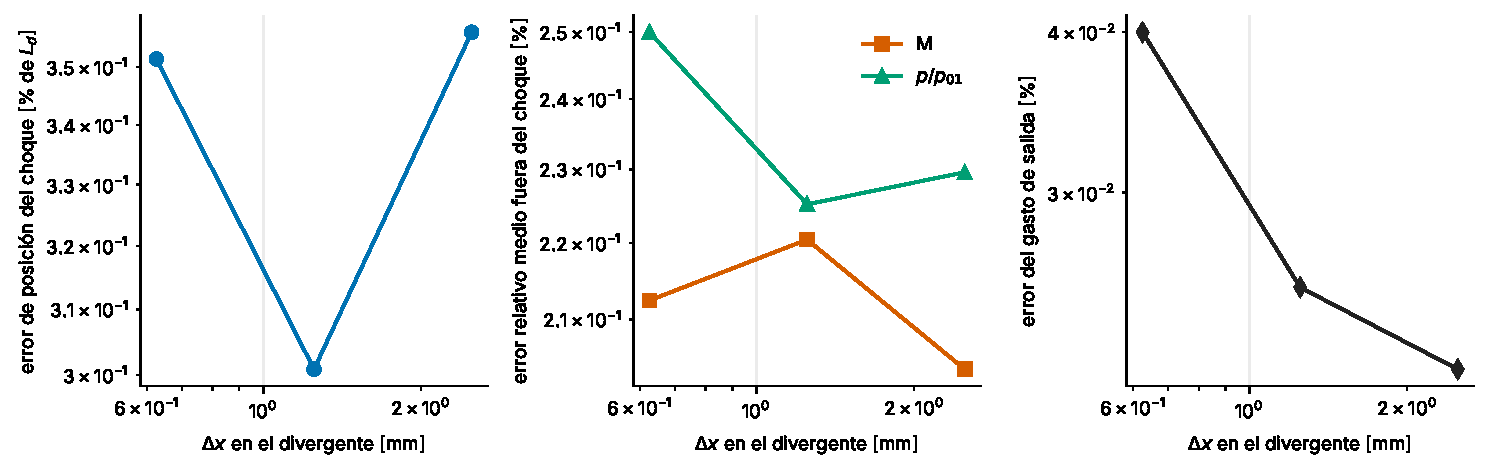
\includegraphics[width=\textwidth]{figuras/convergencia_malla_C.pdf}
  \caption{Estudio de malla del caso C (r1, r2 y r4) en función del tamaño de celda $\Delta x$ en el divergente. Izquierda: error de posición del choque (porcentaje de $L_d$). Centro: error relativo medio de $M$ y $p/p_{01}$ fuera de la zona del choque. Derecha: error del gasto de salida. Los ejes verticales están ampliados: todos los errores son menores de 0.4\,\% de $L_d$, de 0.3\,\% en $M$ y $p/p_{01}$ y de 0.04\,\% en el gasto, sin tendencia monótona al refinar, es decir, los resultados son independientes de la malla a este nivel.}
  \label{fig:conv-malla-C}
\end{figure}

\begin{figure}[htbp]
  \centering
  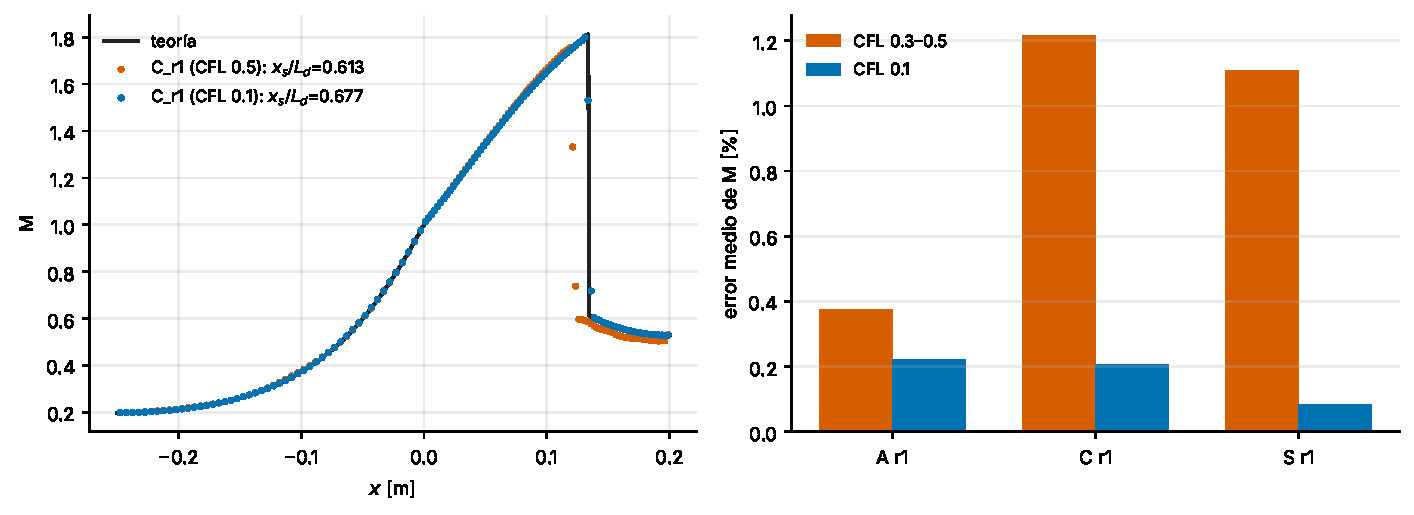
\includegraphics[width=\textwidth]{figuras/sensibilidad_dt.pdf}
  \caption{Sensibilidad al número de CFL. Izquierda: perfil de Mach del caso C (r1) con CFL 0.5 y 0.1; con CFL alto el choque queda desplazado aguas arriba ($x_s/L_d=0.613$) frente al valor con CFL 0.1 (0.677). Derecha: error medio del número de Mach en los casos A, C y S con CFL 0.3--0.5 y con CFL 0.1.}
  \label{fig:sens-dt}
\end{figure}
